%==================== PARTE 1 ====================
\section{O circuito e os valores medidos}
O circuito é de três estágios RC acoplados, com $R_4$ ligado ao terra:
\[
\Vin \;-\; R_1 \;-\; \underbrace{\Vc1}_{C_1} \;-\; R_2 \;-\; \underbrace{\Vc2}_{C_2} \;-\; R_3 \;-\; \underbrace{\Vc3}_{C_3} \;-\; R_4 \;-\; \text{terra}
\]
Valores medidos com o multímetro:
\begin{center}
\begin{tabular}{cccc|ccc}
\toprule $R_1$ & $R_2$ & $R_3$ & $R_4$ & $C_1$ & $C_2$ & $C_3$\\ \midrule
22,0 k$\Omega$ & 46,8 k$\Omega$ & 32,6 k$\Omega$ & 66,8 k$\Omega$ & 947 $\mu$F & 947 $\mu$F & 955 $\mu$F\\ \bottomrule
\end{tabular}
\end{center}

\subsection{Condutâncias}
\begin{formula}\[ g_k=\frac{1}{R_k} \]\end{formula}
\begin{just}Trabalhar com condutâncias evita frações aninhadas: a corrente num resistor é simplesmente $g\cdot\Delta V$.\end{just}
\begin{align*}
g_1&=\frac{1}{22\,000}=45{,}455\ \mu\mathrm{S}, & g_2&=\frac{1}{46\,800}=21{,}368\ \mu\mathrm{S},\\
g_3&=\frac{1}{32\,600}=30{,}675\ \mu\mathrm{S}, & g_4&=\frac{1}{66\,800}=14{,}970\ \mu\mathrm{S}.
\end{align*}
Somas que vão aparecer nas equações (cada nó soma as condutâncias dos dois resistores ligados a ele):
\begin{align*}
A_1&=g_1+g_2=45{,}455+21{,}368=66{,}822\ \mu\mathrm{S}\\
A_2&=g_2+g_3=21{,}368+30{,}675=52{,}042\ \mu\mathrm{S}\\
A_3&=g_3+g_4=30{,}675+14{,}970=45{,}645\ \mu\mathrm{S}
\end{align*}

%------------------------------------------------------------------
\section{Modelo matemático completo (funções de transferência da 1ª avaliação)}
\subsection{Equações dos nós (leis de Kirchhoff das correntes)}
\begin{formula}
Em cada nó: \emph{corrente que chega pelo resistor da esquerda = corrente que vai ao capacitor + corrente que sai pelo resistor da direita}, com $i_C=C\,\dfrac{dv}{dt}$ e $i_R=\dfrac{\Delta V}{R}$.
\end{formula}
\begin{align}
C_1\dot V_{c1}&=\frac{\Vin-\Vc1}{R_1}-\frac{\Vc1-\Vc2}{R_2}\\
C_2\dot V_{c2}&=\frac{\Vc1-\Vc2}{R_2}-\frac{\Vc2-\Vc3}{R_3}\\
C_3\dot V_{c3}&=\frac{\Vc2-\Vc3}{R_3}-\frac{\Vc3-0}{R_4}
\end{align}
\begin{just}O nó 3 só tem $R_4$ para o terra (por isso a tensão do terra é 0). Não existe um quarto capacitor: o sistema tem 3 estados ($\Vc1,\Vc2,\Vc3$), logo é de 3ª ordem.\end{just}

\subsection{Transformada de Laplace}
\begin{just}O circuito é linear e invariante no tempo. Trabalhando com desvios em torno de um ponto de operação (condições iniciais nulas), a derivada vira multiplicação por $s$: $\dot V\to sV$. Isso transforma o sistema diferencial num sistema algébrico.\end{just}
Substituindo $1/R_k=g_k$ e agrupando os termos de cada tensão:
\begin{align*}
(C_1s+g_1+g_2)\,\Vc1-g_2\,\Vc2&=g_1\,\Vin\\
-g_2\,\Vc1+(C_2s+g_2+g_3)\,\Vc2-g_3\,\Vc3&=0\\
-g_3\,\Vc2+(C_3s+g_3+g_4)\,\Vc3&=0
\end{align*}
Definindo $a_{11}=C_1s+A_1$, $a_{22}=C_2s+A_2$, $a_{33}=C_3s+A_3$, em forma matricial $M(s)\mathbf V=\mathbf b\,\Vin$:
\[
\begin{bmatrix}a_{11}&-g_2&0\\-g_2&a_{22}&-g_3\\0&-g_3&a_{33}\end{bmatrix}
\begin{bmatrix}\Vc1\\\Vc2\\\Vc3\end{bmatrix}=\begin{bmatrix}g_1\\0\\0\end{bmatrix}\Vin .
\]

\subsection{Determinante $\Delta(s)=\det M(s)$ (polinômio característico)}
Expansão pela primeira linha:
\[
\Delta=a_{11}\,(a_{22}a_{33}-g_3^2)-(-g_2)\big[(-g_2)a_{33}-(-g_3)\cdot0\big]=a_{11}\,(a_{22}a_{33}-g_3^2)-g_2^2\,a_{33}.
\]
Chamo $P(s)=a_{22}a_{33}-g_3^2$ e expando $(C_2s+A_2)(C_3s+A_3)=C_2C_3s^2+(C_2A_3+C_3A_2)s+A_2A_3$:
\[
P(s)=P_2s^2+P_1s+P_0,\quad P_2=C_2C_3,\;\; P_1=C_2A_3+C_3A_2,\;\; P_0=A_2A_3-g_3^2 .
\]
Substituindo os valores (capacitâncias em F, condutâncias em S):
\begin{align*}
P_2&=947\!\times\!10^{-6}\cdot955\!\times\!10^{-6}=9{,}044\times10^{-7}\\
P_1&=947\!\times\!10^{-6}\cdot45{,}645\!\times\!10^{-6}+955\!\times\!10^{-6}\cdot52{,}042\!\times\!10^{-6}\\&=4{,}323\times10^{-8}+4{,}970\times10^{-8}=9{,}293\times10^{-8}\\
P_0&=52{,}042\!\times\!10^{-6}\cdot45{,}645\!\times\!10^{-6}-(30{,}675\!\times\!10^{-6})^2\\&=2{,}3755\times10^{-9}-9{,}410\times10^{-10}=1{,}435\times10^{-9}
\end{align*}
Agora $\Delta=(C_1s+A_1)P(s)-g_2^2(C_3s+A_3)$. Multiplicando e agrupando por potências de $s$: $\Delta=D_3s^3+D_2s^2+D_1s+D_0$,
\begin{align*}
D_3&=C_1P_2=947\!\times\!10^{-6}\cdot9{,}044\!\times\!10^{-7}=8{,}565\times10^{-10}\\
D_2&=C_1P_1+A_1P_2=8{,}800\times10^{-11}+6{,}043\times10^{-11}=1{,}484\times10^{-10}\\
D_1&=C_1P_0+A_1P_1-g_2^2C_3=1{,}358\times10^{-12}+6{,}210\times10^{-12}-4{,}360\times10^{-13}=7{,}132\times10^{-12}\\
D_0&=A_1P_0-g_2^2A_3=9{,}586\times10^{-14}-2{,}084\times10^{-14}=7{,}502\times10^{-14}
\end{align*}
(onde $g_2^2=4{,}566\times10^{-10}\ \mathrm{S^2}$).

\subsection{Numeradores pela regra de Cramer}
\begin{formula}$V_{cj}=\Delta_j/\Delta$, onde $\Delta_j$ é o determinante de $M$ com a coluna $j$ trocada por $\mathbf b\Vin=[g_1\Vin\ 0\ 0]^T$.\end{formula}
\textbf{$\Vc3$ (coluna 3 trocada).} Expandindo pela terceira coluna (só o 1º elemento é não nulo):
\[
\Delta_3=g_1\Vin\det\begin{bmatrix}-g_2&a_{22}\\0&-g_3\end{bmatrix}=g_1\Vin\,(g_2g_3)\ \Rightarrow\ \frac{\Vc3}{\Vin}=\frac{g_1g_2g_3}{\Delta(s)}.
\]
\textbf{$\Vc2$ (coluna 2 trocada).} Só o 1º elemento é não nulo, com sinal $-1$ (posição (1,2)):
\[
\Delta_2=-g_1\Vin\det\begin{bmatrix}-g_2&-g_3\\0&a_{33}\end{bmatrix}=-g_1\Vin(-g_2a_{33})=g_1g_2a_{33}\Vin\ \Rightarrow\ \frac{\Vc2}{\Vin}=\frac{g_1g_2(C_3s+A_3)}{\Delta(s)}.
\]
\textbf{$\Vc1$ (coluna 1 trocada).} Expandindo pela primeira coluna:
\[
\Delta_1=g_1\Vin\det\begin{bmatrix}a_{22}&-g_3\\-g_3&a_{33}\end{bmatrix}=g_1\Vin\,P(s)\ \Rightarrow\ \frac{\Vc1}{\Vin}=\frac{g_1P(s)}{\Delta(s)}.
\]
\begin{just}Os três quocientes têm o \emph{mesmo denominador} $\Delta(s)$: é o polinômio característico da matriz, e por isso as três tensões compartilham os mesmos polos. O que muda é o numerador (os zeros).\end{just}

\subsection{Normalização (termo constante igual a 1)}
\begin{just}A forma padrão de função de transferência para processos é $K\,\dfrac{\prod(\tau_{z}s+1)}{\prod(\tau_{p}s+1)}$: o termo independente de $s$ vale 1, e o ganho estático $K$ aparece explicitamente. Para chegar lá, divido numerador e denominador por $D_0$ (o termo independente de $\Delta$).\end{just}
\[
\frac{\Delta}{D_0}=\frac{D_3}{D_0}s^3+\frac{D_2}{D_0}s^2+\frac{D_1}{D_0}s+1=\frac{8{,}565\times10^{-10}}{7{,}502\times10^{-14}}s^3+\frac{1{,}484\times10^{-10}}{7{,}502\times10^{-14}}s^2+\frac{7{,}132\times10^{-12}}{7{,}502\times10^{-14}}s+1
\]
\[
D(s)=11\,416{,}7\,s^3+1978{,}65\,s^2+95{,}071\,s+1 .
\]
\begin{res}
\[\frac{\Vc3}{\Vin}=\frac{0{,}3971}{11\,416{,}7\,s^3+1978{,}65\,s^2+95{,}071\,s+1}\]
\[\frac{\Vc2}{\Vin}=\frac{0{,}5910\,(20{,}92\,s+1)}{D(s)},\qquad \frac{\Vc1}{\Vin}=\frac{0{,}8692\,(630{,}4\,s^2+64{,}78\,s+1)}{D(s)}\]
\end{res}
Como os numeradores foram obtidos:
\begin{itemize}
\item $\Vc3$: $\dfrac{g_1g_2g_3}{D_0}=\dfrac{45{,}455\cdot21{,}368\cdot30{,}675\times10^{-18}}{7{,}502\times10^{-14}}=\dfrac{2{,}979\times10^{-14}}{7{,}502\times10^{-14}}=0{,}3971$.
\item $\Vc2$: $\dfrac{g_1g_2(C_3s+A_3)}{D_0}=\dfrac{g_1g_2A_3}{D_0}\left(\dfrac{C_3}{A_3}s+1\right)$; $\dfrac{g_1g_2A_3}{D_0}=\dfrac{4{,}433\times10^{-14}}{7{,}502\times10^{-14}}=0{,}5910$ e $\dfrac{C_3}{A_3}=\dfrac{955\times10^{-6}}{45{,}645\times10^{-6}}=20{,}92$ s.
\item $\Vc1$: $\dfrac{g_1P(s)}{D_0}=\dfrac{g_1P_0}{D_0}\left(\dfrac{P_1}{P_0}s+\dfrac{P_2}{P_0}s^2+1\right)$; $\dfrac{g_1P_0}{D_0}=\dfrac{6{,}520\times10^{-14}}{7{,}502\times10^{-14}}=0{,}8692$, $\dfrac{P_1}{P_0}=\dfrac{9{,}293\times10^{-8}}{1{,}435\times10^{-9}}=64{,}78$, $\dfrac{P_2}{P_0}=\dfrac{9{,}044\times10^{-7}}{1{,}435\times10^{-9}}=630{,}4$.
\end{itemize}

\subsection{Ganhos estáticos (duas conferências)}
O ganho estático é $G(0)$. Pelo método anterior: $K_3=0{,}3971$, $K_2=0{,}5910$, $K_1=0{,}8692$.

\textbf{Conferência por divisores resistivos.} Em regime permanente os capacitores são circuitos abertos (corrente nula), então a mesma corrente $\Vin/R_t$ percorre todos os resistores, com $R_t=R_1+R_2+R_3+R_4=22+46{,}8+32{,}6+66{,}8=168{,}2$ k$\Omega$:
\[\begin{gathered}
K_3=\frac{R_4}{R_t}=\frac{66{,}8}{168{,}2}=0{,}3971,\\
K_2=\frac{R_3+R_4}{R_t}=\frac{99{,}4}{168{,}2}=0{,}5910,\\
K_1=\frac{R_2+R_3+R_4}{R_t}=\frac{146{,}2}{168{,}2}=0{,}8692 .
\end{gathered}\]
Os dois caminhos coincidem, o que confirma o modelo.

\subsection{Polos, zeros e constantes de tempo}
As raízes de $D(s)=0$ (cúbica, resolvida numericamente) são
$s_1=-0{,}01456$, $s_2=-0{,}06250$, $s_3=-0{,}09625$ s$^{-1}$.
\begin{formula}Cada polo real $s=-1/\tau_i$ dá uma constante de tempo $\tau_i=-1/s$; o denominador fatora em $(\tau_1s+1)(\tau_2s+1)(\tau_3s+1)$.\end{formula}
\[
\tau_1=\frac{1}{0{,}01456}=68{,}68\ \mathrm{s},\qquad \tau_2=\frac{1}{0{,}06250}=16{,}00\ \mathrm{s},\qquad \tau_3=\frac{1}{0{,}09625}=10{,}39\ \mathrm{s}.
\]
\textbf{Verificação pelas relações de Vieta} (coeficientes do produto $(\tau_1s+1)(\tau_2s+1)(\tau_3s+1)$ devem ser os de $D(s)$):
\begin{align*}
\tau_1+\tau_2+\tau_3&=68{,}68+16{,}00+10{,}39=95{,}07\ \ \checkmark\ (\text{coef. de }s)\\
\tau_1\tau_2+\tau_1\tau_3+\tau_2\tau_3&=1098{,}9+713{,}6+166{,}2=1978{,}7\ \ \checkmark\ (\text{coef. de }s^2)\\
\tau_1\tau_2\tau_3&=68{,}68\cdot16{,}00\cdot10{,}39=11\,416{,}7\ \ \checkmark\ (\text{coef. de }s^3)
\end{align*}
Todas as raízes são reais e negativas $\Rightarrow$ sistema estável e \textbf{sobreamortecido} (sem oscilação). A constante \emph{dominante} é $\tau_1=68{,}68$ s (a maior; é $68{,}68/16{,}00=4{,}29$ vezes a segunda).

\textbf{Zeros (constantes de tempo de avanço):}
\begin{itemize}
\item $\Vc3$: o numerador é constante $\Rightarrow$ não há zeros.
\item $\Vc2$: o zero é a raiz de $C_3s+A_3=0$, isto é, $\tau_z=C_3/A_3=20{,}92$ s.
\item $\Vc1$: os zeros são as raízes de $630{,}4s^2+64{,}78s+1=0$. Por Bhaskara:
\[
\Delta=64{,}78^2-4\cdot630{,}4\cdot1=4196{,}4-2521{,}6=1674{,}8,\quad\sqrt\Delta=40{,}92,
\]
\[
s=\frac{-64{,}78\pm40{,}92}{2\cdot630{,}4}\ \Rightarrow\ s_{z1}=-0{,}01892,\ s_{z2}=-0{,}08383\ \Rightarrow\ \tau_{z1}=52{,}85\ \mathrm{s},\ \tau_{z2}=11{,}93\ \mathrm{s}.
\]
Conferência: $52{,}85\cdot11{,}93=630{,}5$ e $52{,}85+11{,}93=64{,}78$ $\checkmark$.
\end{itemize}
\begin{res}
\begin{align}
\frac{\Vc3}{\Vin}&=\frac{0{,}3971}{(68{,}68s+1)(16{,}00s+1)(10{,}39s+1)}\label{ft3}\\
\frac{\Vc2}{\Vin}&=\frac{0{,}5910\,(20{,}92s+1)}{(68{,}68s+1)(16{,}00s+1)(10{,}39s+1)}\\
\frac{\Vc1}{\Vin}&=\frac{0{,}8692\,(52{,}85s+1)(11{,}93s+1)}{(68{,}68s+1)(16{,}00s+1)(10{,}39s+1)}
\end{align}
\end{res}
\begin{just}\textbf{Tipo de curva previsto pelo grau relativo} (polos $-$ zeros): $\Vc1$ tem $3-2=1$, então a derivada em $t=0^+$ é diferente de zero e a curva tem inclinação máxima logo no início (\textbf{curva tipo C}). $\Vc2$ tem $3-1=2$ e $\Vc3$ tem $3-0=3$: a inclinação inicial é nula e há ponto de inflexão (\textbf{curva tipo S}). Isso diz de antemão qual método de redução usar em cada tensão. O sistema é \emph{interativo}: as constantes de tempo (10,4; 16,0; 68,7 s) são bem diferentes das de cada estágio isolado ($R_1C_1=20{,}8$ s etc.), porque cada capacitor carrega e descarrega os vizinhos.\end{just}

\subsection{Resposta ao degrau da FT completa (frações parciais)}
\begin{formula}Para $u=U\cdot1(t)$ e $G(s)=K\dfrac{\prod_k(\tau_{z,k}s+1)}{\prod_i(\tau_is+1)}$ com polos distintos:
\[
y(t)=K\Big[1-\sum_{i=1}^{3}c_i\,e^{-t/\tau_i}\Big],\qquad c_i=\frac{\prod_k\left(1-\tau_{z,k}/\tau_i\right)}{\prod_{j\ne i}\left(1-\tau_j/\tau_i\right)}\quad(U=1).\]
\end{formula}
\begin{just}O resíduo da exponencial em $s=-1/\tau_i$ é obtido multiplicando $Y(s)$ por $(\tau_is+1)$ e calculando em $s=-1/\tau_i$. Em $s=0$ o resíduo é $K$ (valor final). Como $y(0)=0$, deve valer $\sum c_i=1$ --- é a conferência.\end{just}
Exemplo detalhado: $\Vc3$, $c_1$ (polo $\tau_1=68{,}68$):
\[
c_1=\frac{1}{(1-\tau_2/\tau_1)(1-\tau_3/\tau_1)}=\frac{1}{(1-0{,}2329)(1-0{,}1513)}=\frac{1}{0{,}7671\cdot0{,}8487}=1{,}536 .
\]
Exemplo $\Vc2$, $c_1$ (numerador com $\tau_z=20{,}92$): $c_1=\dfrac{1-20{,}92/68{,}68}{0{,}7671\cdot0{,}8487}=\dfrac{0{,}6954}{0{,}6510}=1{,}068$. Os demais coeficientes seguem o mesmo procedimento:
\begin{center}
\begin{tabular}{lccc}\toprule & $c_1$ ($\tau_1=68{,}7$) & $c_2$ ($\tau_2=16{,}0$) & $c_3$ ($\tau_3=10{,}4$)\\\midrule
$\Vc3$ & $1{,}5360$ & $-0{,}8662$ & $0{,}3302$\\ $\Vc2$ & $1{,}0681$ & $0{,}2666$ & $-0{,}3347$\\ $\Vc1$ & $0{,}2926$ & $0{,}5075$ & $0{,}1999$\\\bottomrule
\end{tabular}
\end{center}
Conferência $\sum c_i=1$ em cada linha (p.\,ex.\ $\Vc3$: $1{,}5360-0{,}8662+0{,}3302=1{,}0000$). Esta expressão é a ``resposta da FT completa'' usada nas comparações.

%------------------------------------------------------------------
\section{Teste ao degrau experimental}
\subsection{O arquivo e o trecho usado}
O ScadaBR gravou uma amostra por segundo de cinco variáveis (1440 amostras cada): $SO=\Vin$, $VP=\Vc3$, $VP1=\Vc2$, $VP2=\Vc1$ (e $SP$). A entrada \texttt{SO} fica em 30\,\% nos primeiros 41 s, em 70\,\% até $t=577$ s e depois em 50\,\% até o fim. Para identificar as FTs reduzidas usei \textbf{apenas o degrau de 70\,\% para 50\,\%}:
\[
\Delta U=U_1-U_0=50{,}000-70{,}001=-20{,}000\,\%\ (\approx-1\ \mathrm{V}),\qquad t_{degrau}=576{,}5\ \mathrm{s}.
\]
\begin{just}O degrau começa de um regime permanente real (o patamar de 70\,\% dura 535 s, mais de $7\tau_1=481$ s) e termina em outro patamar longo (863 s). Assim $y_i$ e $y_f$ são confiáveis e não há transitório de teste anterior contaminando. Como o circuito é linear, o resultado vale para qualquer ponto de operação e para degraus em qualquer sentido.\end{just}
\begin{figure}[H]\centering
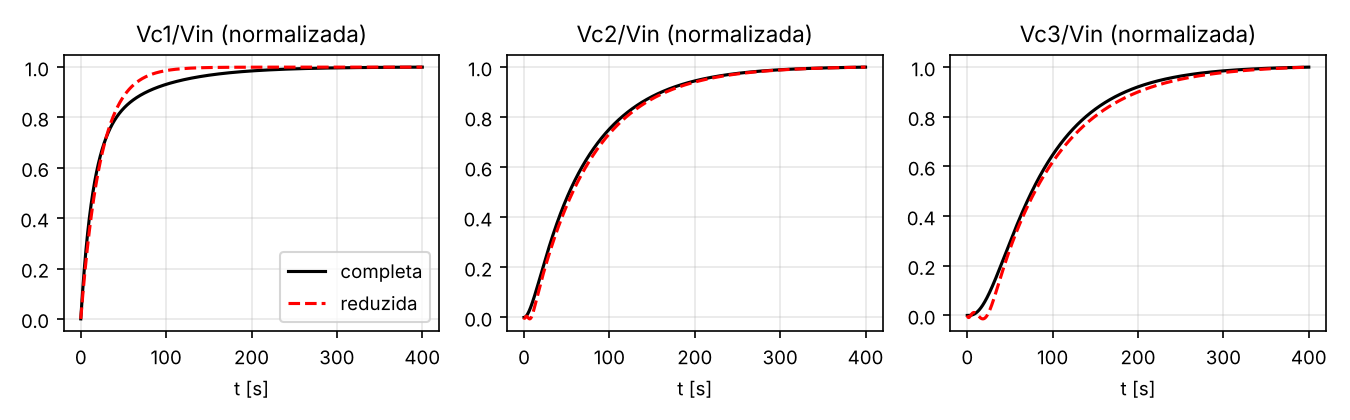
\includegraphics[width=.8\textwidth]{figs/steps.png}
\caption{Respostas ao degrau normalizadas das FTs completas (preto) e das reduzidas (vermelho tracejado), calculadas neste documento.}\end{figure}

\subsection{Tratamento dos dados}
\begin{formula}
$\displaystyle y_n(t)=\frac{y(t)-y_i}{y_f-y_i}$ (resposta normalizada, vai de 0 a 1);\qquad $\displaystyle K=\frac{y_f-y_i}{\Delta U}$.
\end{formula}
\begin{just}Normalizar elimina o sinal negativo do degrau (queda de 70 para 50) e permite aplicar as fórmulas dos métodos como se fosse um degrau positivo unitário. $y_i$ é a média das 128 amostras antes do degrau; $y_f$, a média das 150 últimas amostras (médias reduzem o ruído de quantização do ADC de 10 bits, resolução $100/1024=0{,}0977\,\%$).\end{just}
\begin{center}
\begin{tabular}{lccc}\toprule & $\Vc1$ & $\Vc2$ & $\Vc3$\\\midrule
$y_i$ [\%] (SO=70\,\%) & 60,774 & 41,104 & 27,454\\
$y_f$ [\%] (SO=50\,\%) & 43,431 & 29,382 & 19,618\\
$y_f-y_i$ [\%] & $-17{,}343$ & $-11{,}723$ & $-7{,}836$\\\bottomrule
\end{tabular}
\end{center}
\[
K_1=\frac{-17{,}343}{-20}=0{,}8671,\qquad K_2=\frac{-11{,}723}{-20}=0{,}5861,\qquad K_3=\frac{-7{,}836}{-20}=0{,}3918 .
\]
\textbf{Conferência pelo patamar final:} $y_f/50$: $43{,}431/50=0{,}8686$; $29{,}382/50=0{,}5876$; $19{,}618/50=0{,}3924$ (praticamente iguais, confirmando linearidade: saída nula para entrada nula).
\textbf{Comparação com a teoria:} o ganho medido fica 0,2\,\% a 1,3\,\% abaixo ($0{,}8671$ vs.\ $0{,}8692$; $0{,}5861$ vs.\ $0{,}5910$; $0{,}3918$ vs.\ $0{,}3971$), coerente com as tolerâncias dos $R$ e $C$, a quantização do ADC e a resistência de saída do Arduino. Adoto $K=(y_f-y_i)/\Delta U$, de modo que a FT reduzida termina exatamente no valor final medido.

\subsection{Instantes de 28,3\,\%, 35,3\,\%, 63,2\,\% e 85,3\,\%}
\begin{formula}Para cada nível $q$, procuro a primeira amostra $k+1$ com $y_n\ge q$ e interpolo linearmente entre $k$ e $k+1$:
\[t_q=t_k+\frac{q-y_{n,k}}{y_{n,k+1}-y_{n,k}}(t_{k+1}-t_k).\]\end{formula}
Exemplo completo ($\Vc3$, $q=0{,}632$): $t_k=103{,}5$ s ($y_{n,k}=0{,}6264$) e $t_{k+1}=104{,}5$ s ($y_{n,k+1}=0{,}6388$):
\[
t_{63,2}=103{,}5+\frac{0{,}632-0{,}6264}{0{,}6388-0{,}6264}\,(104{,}5-103{,}5)=103{,}5+\frac{0{,}0056}{0{,}0124}\cdot1=103{,}5+0{,}45=103{,}95\ \mathrm{s}.
\]
Resultados (em segundos desde o degrau):
\begin{center}
\begin{tabular}{lcccc}\toprule & $t_{28,3}$ & $t_{35,3}$ & $t_{63,2}$ & $t_{85,3}$\\\midrule
$\Vc1$ & 7,16 & 9,31 & 23,31 & 58,39\\ $\Vc2$ & 32,34 & 39,12 & 78,26 & 146,80\\ $\Vc3$ & 51,93 & 60,55 & 103,95 & 173,70\\\bottomrule
\end{tabular}
\end{center}

%------------------------------------------------------------------
\section{Redução a ganho, constante de tempo e atraso}
\subsection{O modelo reduzido e a origem dos métodos}
\begin{formula}Modelo de 1ª ordem com atraso (FOPDT): $\displaystyle G(s)=\frac{K\,e^{-t_0s}}{\tau s+1}$. Sua resposta ao degrau é $y_n(t)=1-e^{-(t-t_0)/\tau}$ para $t\ge t_0$ (e $0$ antes).\end{formula}
Cada método de identificação vem de impor que essa curva passe por pontos da curva real. Vou deduzir as constantes numéricas para entender de onde saem.

\textbf{Curva tipo C} (sem inflexão, inclinação máxima na origem; caso de $\Vc1$): não há atraso, $t_0=0$, e em $t=\tau$ a resposta vale $1-e^{-1}=0{,}632$. Logo $\tau=t_{63,2}$.

\textbf{Curva tipo S, método de Smith (Ajuste 3, seção 7-2.1 do livro).} Impondo que a FOPDT passe pelos pontos de 28,3\,\% e 63,2\,\%:
\[\begin{gathered}
1-e^{-(t_{28,3}-t_0)/\tau}=0{,}283\ \Rightarrow\ \frac{t_{28,3}-t_0}{\tau}=-\ln(0{,}717)=0{,}333\approx\frac13,\\
1-e^{-(t_{63,2}-t_0)/\tau}=0{,}632\ \Rightarrow\ \frac{t_{63,2}-t_0}{\tau}=1 .
\end{gathered}\]
Subtraindo: $t_{63,2}-t_{28,3}=\tau(1-\tfrac13)=\tfrac23\tau$. Logo
\[
\boxed{\tau=1{,}5\,(t_{63,2}-t_{28,3}),\qquad t_0=t_{63,2}-\tau .}
\]
\textbf{Método de Sundaresan--Krishnaswamy} (mesmo raciocínio com 35,3\,\% e 85,3\,\%):
$\frac{t_{35,3}-t_0}{\tau}=-\ln(0{,}647)=0{,}435$ e $\frac{t_{85,3}-t_0}{\tau}=-\ln(0{,}147)=1{,}917$. Subtraindo: $t_{85,3}-t_{35,3}=1{,}482\tau$, logo $\tau=0{,}675\,(t_{85,3}-t_{35,3})\approx0{,}67(t_{85,3}-t_{35,3})$ e $t_0=t_{35,3}-0{,}435\tau=1{,}3\,t_{35,3}-0{,}29\,t_{85,3}$.

\textbf{Método da tangente no ponto de inflexão (Ziegler--Nichols, Ajuste 1).} Acho o ponto de maior inclinação $(t_i,y_i)$ com inclinação $m$. A reta tangente $y=y_i+m(t-t_i)$ corta o eixo do tempo ($y=0$) em $t_0=t_i-y_i/m$ e atinge o valor final ($y=1$) em $t=t_i+(1-y_i)/m$; então $\tau=\big[t_i+(1-y_i)/m\big]-t_0$.

\subsection{Contas, passo a passo}
\textbf{$\Vc1$ (tipo C).} A inclinação máxima ocorre na primeira amostra ($m=0{,}0500$ s$^{-1}$; a derivada teórica em $0^+$ é $0{,}048$ s$^{-1}$, ver Lista 2). Então $t_0=0$ e $\tau=t_{63,2}=23{,}31$ s. \emph{Teste de coerência:} se eu tentasse Smith, $\tau=1{,}5(23{,}31-7{,}16)=24{,}23$ s e $t_0=23{,}31-24{,}23=-0{,}92$ s: atraso \emph{negativo}, sem sentido físico (a saída não antecipa a entrada), o que confirma que não há atraso.

\textbf{$\Vc2$ (tipo S), Smith:}
\[
\tau=1{,}5\,(78{,}26-32{,}34)=1{,}5\cdot45{,}92=68{,}88\ \mathrm{s},\qquad t_0=78{,}26-68{,}88=9{,}38\ \mathrm{s}.
\]
\textbf{$\Vc3$ (tipo S), Smith:}
\[
\tau=1{,}5\,(103{,}95-51{,}93)=1{,}5\cdot52{,}02=78{,}03\ \mathrm{s},\qquad t_0=103{,}95-78{,}03=25{,}92\ \mathrm{s}.
\]
\textbf{Sundaresan:} $\Vc2$: $\tau=0{,}67(146{,}80-39{,}12)=72{,}15$ s, $t_0=1{,}3\cdot39{,}12-0{,}29\cdot146{,}80=50{,}86-42{,}57=8{,}29$ s. $\Vc3$: $\tau=0{,}67(173{,}70-60{,}55)=75{,}81$ s, $t_0=1{,}3\cdot60{,}55-0{,}29\cdot173{,}70=78{,}72-50{,}37=28{,}35$ s.

\textbf{Tangente} (pontos de inflexão medidos): $\Vc2$: $t_i=22{,}5$, $y_i=0{,}178$, $m=0{,}01151$ s$^{-1}$: $t_0=22{,}5-0{,}178/0{,}01151=7{,}07$ s; $\tau=\big[22{,}5+(1-0{,}178)/0{,}01151\big]-7{,}07=93{,}93-7{,}07=86{,}86$ s. $\Vc3$: $t_i=43{,}5$, $y_i=0{,}213$, $m=0{,}00884$: $t_0=43{,}5-24{,}10=19{,}38$ s; $\tau=\big[43{,}5+0{,}787/0{,}00884\big]-19{,}38=132{,}5-19{,}38=113{,}10$ s.

\subsection{Resultados e escolha do método}
\begin{center}\small
\begin{tabular}{lccc}\toprule $\tau/t_0$ [s] & $\Vc1$ & $\Vc2$ & $\Vc3$\\\midrule
Tipo C ($\tau=t_{63,2}$, $t_0=0$) & \textbf{23,3 / 0,0} & 78,3 / 0,0 & 104,0 / 0,0\\
Smith (28,3/63,2) & 24,2 / $-0{,}9$ & \textbf{68,9 / 9,4} & \textbf{78,0 / 25,9}\\
Sundaresan (35,3/85,3) & 32,9 / $-4{,}8$ & 72,1 / 8,3 & 75,8 / 28,3\\
Tangente (Z--N) & 20,0 / 0,6 & 86,9 / 7,1 & 113,1 / 19,4\\
Mínimos quadrados (referência) & 27,0 / 0,0 & 72,1 / 7,5 & 79,7 / 23,4\\\bottomrule
\end{tabular}\end{center}
Para comparar os modelos com o experimento uso o erro RMS e o erro máximo, em \% do degrau:
\[
\begin{gathered}\varepsilon_{rms}=100\sqrt{\frac1N\sum_{k=1}^{N}\big(y_{mod,n}(t_k)-y_{exp,n}(t_k)\big)^2},\\
\varepsilon_{max}=100\max_k|y_{mod,n}(t_k)-y_{exp,n}(t_k)|,\quad 0<t<520\,\mathrm{s}\ (N=520).\end{gathered}
\]
RMS (máximo), vindos do relatório original com os dados:
\begin{center}\small
\begin{tabular}{lccc}\toprule & $\Vc1$ & $\Vc2$ & $\Vc3$\\\midrule
Tipo C & 2,87 (7,3) & 1,89 (8,5) & 4,89 (15,6)\\
Smith & 2,71 (6,8) & 0,71 (4,1) & 1,12 (7,1)\\
Sundaresan & 3,28 (13,3) & 0,53 (3,2) & 1,45 (9,1)\\
Tangente & 3,67 (9,4) & 3,55 (7,5) & 6,71 (12,6)\\
Mínimos quadrados & 2,48 (7,2) & 0,44 (2,6) & 0,97 (5,3)\\
FT completa & 0,73 (3,5) & 1,48 (3,2) & 1,75 (3,6)\\\bottomrule
\end{tabular}\end{center}
\begin{just}\textbf{$\Vc1$:} é curva tipo C (Smith dá atraso negativo), logo $\tau=t_{63,2}$ e $t_0=0$. \textbf{$\Vc2$ e $\Vc3$:} adoto Smith porque (i) é o método do livro (Ajuste 3); (ii) usa dois pontos no meio da subida, pouco sensíveis à quantização e ao valor final; (iii) seu erro RMS fica próximo ao dos mínimos quadrados (o melhor possível para uma FOPDT). A tangente é a pior (RMS 6,7\,\% em $\Vc3$): a inclinação máxima de um sistema de 3ª ordem é muito sensível à suavização dos dados. Tratar $\Vc3$ como curva C (RMS 4,9\,\%) também é ruim, o que confirma que ela é do tipo S.\end{just}
\textbf{Conferência independente (regra prática do livro, p.\,216):} $\tau\approx$ maior constante de tempo, $t_0\approx$ soma das menores. Com a Seção 2: $\tau\approx68{,}7$ s e $t_0\approx16{,}0+10{,}4=26{,}4$ s, próximo do identificado para $\Vc3$ ($78{,}0$ s e $25{,}9$ s).
\begin{res}
\[
\frac{\Vc1}{\Vin}\approx\frac{0{,}867}{23{,}3s+1},\qquad
\frac{\Vc2}{\Vin}\approx\frac{0{,}586\,e^{-9{,}4s}}{68{,}9s+1},\qquad
\frac{\Vc3}{\Vin}\approx\frac{0{,}392\,e^{-25{,}9s}}{78{,}0s+1}\ \ \text{(a planta de controle)}
\]
\end{res}

%------------------------------------------------------------------
\section{Comparação das respostas ao degrau}
A figura da Seção 3 já mostra as respostas normalizadas; os erros RMS acima quantificam: a FT completa acompanha o experimento com RMS de 0,7\,\% a 1,7\,\% do degrau (valida o modelo físico e as medidas de $R$ e $C$); a reduzida erra mais (2,9\,\% em $\Vc1$, 0,7\,\% em $\Vc2$, 1,1\,\% em $\Vc3$), o que é esperado: troca 3 polos (e zeros) por 1 polo e 1 atraso. Em $\Vc3$ e $\Vc2$ a reduzida reproduz o atraso inicial e a subida; a maior diferença está na cauda, pois o 1º ordem não representa o peso diferente do polo lento ($\tau_1=68{,}7$ s). Em $\Vc1$ a reduzida fica próxima da curva real até $\sim$20 s, cruza e depois fica acima, porque $\Vc1$ não é naturalmente de 1ª ordem (tem 3 polos e 2 zeros).

%------------------------------------------------------------------
\section{Diagramas de Bode e margens}
\subsection{Respostas em frequência}
\begin{formula}Substituindo $s=j\omega$ em $G(s)=K\prod(\tau_{z}s+1)/\prod(\tau_ps+1)$ e $G_{red}=Ke^{-t_0s}/(\tau s+1)$:
\[
|G_{compl}(j\omega)|=K\frac{\prod_k\sqrt{1+(\omega\tau_{z,k})^2}}{\prod_i\sqrt{1+(\omega\tau_i)^2}},\qquad
\angle G_{compl}=\sum_k\arctan(\omega\tau_{z,k})-\sum_i\arctan(\omega\tau_i),
\]
\[
|G_{red}(j\omega)|=\frac{K}{\sqrt{1+(\omega\tau)^2}},\qquad\angle G_{red}=-\arctan(\omega\tau)-\omega t_0\ (\text{rad}).
\]\end{formula}
\begin{just}O módulo de $(\tau s+1)$ em $s=j\omega$ é $\sqrt{1+\omega^2\tau^2}$ e sua fase é $\arctan(\omega\tau)$; polos entram no denominador (subtraem fase), zeros no numerador (somam fase). O atraso puro $e^{-j\omega t_0}$ tem módulo 1 e fase $-\omega t_0$, que decresce sem limite com $\omega$ --- por isso a FOPDT difere tanto da completa em alta frequência.\end{just}
\textbf{Exemplo numérico completo: $\Vc3$ em $\omega=0{,}1$ rad/s.} FT completa:
\begin{align*}
\sqrt{1+(0{,}1\cdot68{,}68)^2}&=\sqrt{1+47{,}17}=6{,}941, & \arctan(6{,}868)&=81{,}72^\circ\\
\sqrt{1+(0{,}1\cdot16{,}00)^2}&=\sqrt{1+2{,}56}=1{,}887, & \arctan(1{,}600)&=57{,}99^\circ\\
\sqrt{1+(0{,}1\cdot10{,}39)^2}&=\sqrt{1+1{,}079}=1{,}442, & \arctan(1{,}039)&=46{,}10^\circ
\end{align*}
\[
|G|=\frac{0{,}3971}{6{,}941\cdot1{,}887\cdot1{,}442}=\frac{0{,}3971}{18{,}89}=0{,}0210,\qquad \angle G=-(81{,}72+57{,}99+46{,}10)=-185{,}8^\circ .
\]
FT reduzida: $\sqrt{1+(0{,}1\cdot78{,}03)^2}=\sqrt{1+60{,}89}=7{,}867$, $|G|=0{,}3918/7{,}867=0{,}0498$; fase $=-\arctan(7{,}803)-0{,}1\cdot25{,}92\ \mathrm{rad}=-82{,}70^\circ-148{,}52^\circ=-231{,}2^\circ$ (o atraso contribui com $\omega t_0=2{,}592\ \mathrm{rad}=148{,}5^\circ$).

\begin{figure}[H]\centering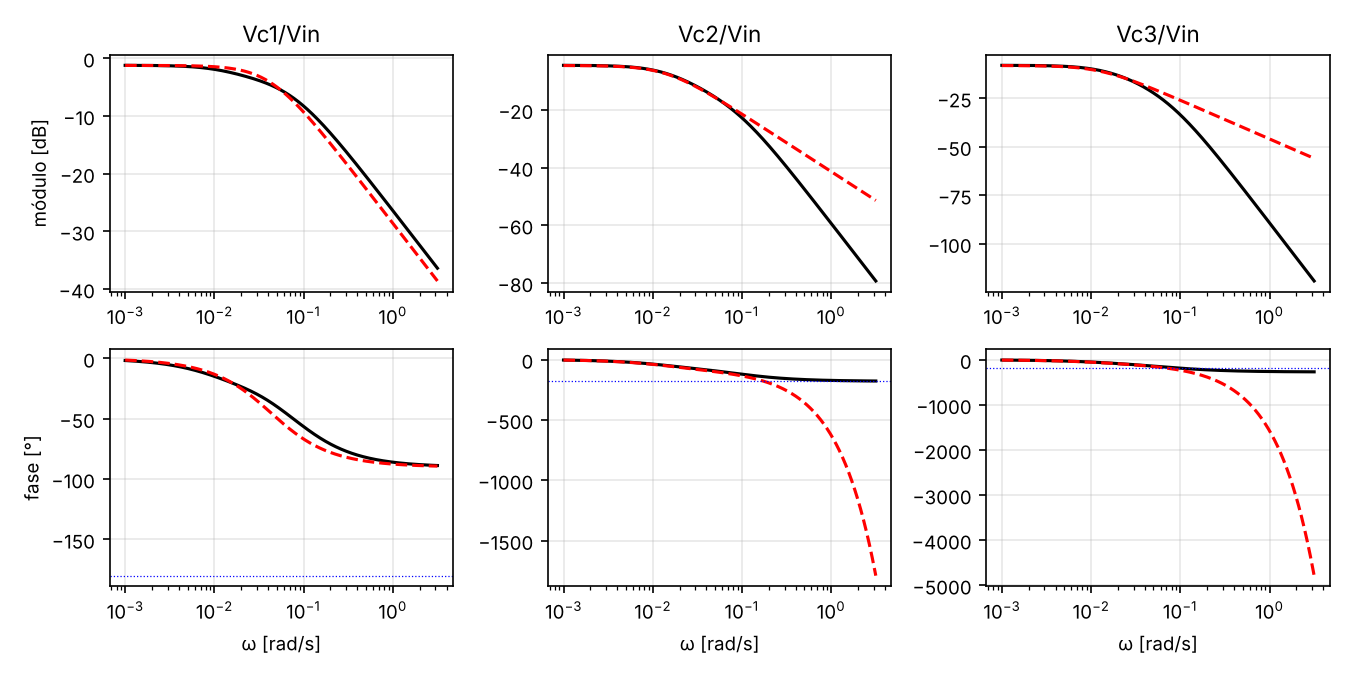
\includegraphics[width=.95\textwidth]{figs/bode.png}
\caption{Bode das FTs completas (preto) e reduzidas (vermelho tracejado).}\end{figure}
Valores em algumas frequências (módulo e fase em graus):
\begin{center}\small
\begin{tabular}{c|cc|cc|cc}\toprule
 & \multicolumn{2}{c|}{$\Vc1$ completa / reduzida} & \multicolumn{2}{c|}{$\Vc2$ completa} & \multicolumn{2}{c}{$\Vc3$ completa / reduzida}\\
$\omega$ [rad/s] & $|G|$ & $\angle G$ & $|G|$ & $\angle G$ & $|G|$ & $\angle G$ / red.\\\midrule
0,01 & 0,8016 (red 0,8445) & $-14{,}8$ ($-13{,}1$) & 0,4888 & $-37{,}7$ & 0,3215 & $-49{,}5$ ($-52{,}8$)\\
0,03 & 0,6503 (0,7106) & $-29{,}6$ ($-35{,}0$) & 0,2622 & $-74{,}9$ & 0,1492 & $-107{,}1$ ($-111{,}4$)\\
0,10 & 0,3854 (0,3419) & $-56{,}5$ ($-66{,}8$) & 0,0726 & $-121{,}3$ & 0,0210 & $-185{,}8$ ($-231{,}2$)\\
0,30 & 0,1550 (0,1228) & $-76{,}9$ ($-81{,}9$) & 0,0113 & $-156{,}7$ & 0,0012 & $-237{,}7$ ($-533{,}1$)\\\bottomrule
\end{tabular}\end{center}

\subsection{Margens de ganho e de fase}
Como $K<1$ em todas as plantas, o módulo da planta sozinha nunca chega a 0 dB: não existe cruzamento de ganho e a margem de fase seria infinita. Para obter margens com significado, fecho a malha com um controlador proporcional $K_c$ e comparo:
\begin{itemize}
\item o \textbf{ganho crítico} $K_{cu}=1/|G(j\omega_{180})|$, onde $\omega_{180}$ é a frequência em que a fase vale $-180^\circ$ (margem de ganho da planta);
\item a \textbf{margem de fase} $PM=180^\circ+\angle\big(K_cG(j\omega_g)\big)$, onde $|K_cG(j\omega_g)|=1$, para $K_c=3,5,10$.
\end{itemize}
\textbf{Cálculo exato de $K_{cu}$ para a FT completa de $\Vc3$ (critério de Routh).}
\begin{formula}Com $K_c$ puro, a equação característica é $1+K_cG(s)=0$. Para um polinômio $a_3s^3+a_2s^2+a_1s+a_0=0$, a linha $s^1$ da tabela de Routh é $\big[a_2a_1-a_3a_0\big]/a_2$; a estabilidade marginal ocorre quando essa linha se anula. O polinômio auxiliar é $a_2s^2+a_0=0$.\end{formula}
Aqui $a_3=11\,416{,}7$, $a_2=1978{,}65$, $a_1=95{,}071$, $a_0=1+K_cK_3$:
\[
a_2a_1=a_3(1+K_{cu}K_3)\ \Rightarrow\ 1+K_{cu}K_3=\frac{a_2a_1}{a_3}=\frac{1978{,}65\cdot95{,}071}{11\,416{,}7}=16{,}477
\]
\[
K_{cu}=\frac{16{,}477-1}{0{,}3971}=38{,}97 .
\]
Frequência de oscilação (polinômio auxiliar): $\omega_u^2=a_0/a_2=(1+K_{cu}K_3)/a_2=a_1/a_3$, logo
\[
\omega_u=\sqrt{\frac{95{,}071}{11\,416{,}7}}=\sqrt{0{,}008328}=0{,}09125\ \mathrm{rad/s},\qquad T_u=\frac{2\pi}{\omega_u}=\frac{6{,}2832}{0{,}09125}=68{,}85\ \mathrm{s}.
\]
\textbf{Para a FT reduzida de $\Vc3$.} Resolvo $-\arctan(\omega\tau)-\omega t_0=-\pi$, isto é, $f(\omega)=\pi-\arctan(78{,}03\omega)-25{,}92\omega=0$, por bisseção (em $f>0$ o ponto fica à esquerda da raiz):
\begin{center}\small
\begin{tabular}{cccc}\toprule passo & intervalo & ponto médio & $f$\\\midrule
1 & [0,010; 0,200] & 0,1050 & $-1{,}029$\\ 2 & [0,010; 0,1050] & 0,0575 & $+0{,}300$\\ 3 & [0,0575; 0,1050] & 0,0813 & $-0{,}379$\\ 4 & [0,0575; 0,0813] & 0,0694 & $-0{,}045$\\ 5 & [0,0575; 0,0694] & 0,0634 & $+0{,}126$\\ 6 & [0,0634; 0,0694] & 0,0664 & $+0{,}040$\\ $\vdots$ & & & \\\bottomrule
\end{tabular}\end{center}
Convergindo: $\omega_{180}=0{,}0678$ rad/s. Verificação: $\arctan(0{,}0678\cdot78{,}03=5{,}290)=79{,}3^\circ=1{,}384$ rad e $\omega t_0=0{,}0678\cdot25{,}92=1{,}757$ rad; soma $=3{,}141$ rad $=\pi$ $\checkmark$. Então
\[
K_{cu}=\frac{\sqrt{1+(\omega_{180}\tau)^2}}{K}=\frac{\sqrt{1+5{,}290^2}}{0{,}3918}=\frac{5{,}383}{0{,}3918}=13{,}74 .
\]
Para $\Vc2$ reduzida o mesmo procedimento dá $\omega_{180}=0{,}176$ rad/s e $K_{cu}=20{,}8$.

\textbf{$\Vc1$ e $\Vc2$ completas.} $\Vc1$ (3 polos, 2 zeros): a fase fica entre $0^\circ$ e $-90^\circ$, nunca chega a $-180^\circ$: $K_{cu}$ não existe. $\Vc2$ (3 polos, 1 zero): a fase tende a $-180^\circ$ por cima sem atingi-la (confirmado no gráfico e por Routh: a linha $s^1$ fica $a_2(a_1+K_cK_2\tau_z)-a_3(1+K_cK_2)>0$ para todo $K_c$, pois $a_2\tau_z>a_3$), também sem $K_{cu}$ finito.

\textbf{Margem de fase, exemplo completo ($\Vc3$ completa, $K_c=5$).} Procuro $\omega_g$ tal que $5|G(j\omega_g)|=1$, isto é, $|G|=0{,}2$. Por tentativa numérica: $\omega_g=0{,}0222$ rad/s. Fase nesse ponto:
\[
-\big[\arctan(0{,}0222\cdot68{,}68)+\arctan(0{,}0222\cdot16{,}00)+\arctan(0{,}0222\cdot10{,}39)\big]=-(56{,}7+19{,}5+13{,}0)=-89{,}3^\circ,
\]
\[
PM=180^\circ-89{,}3^\circ=90{,}7^\circ .
\]
\begin{center}
\begin{tabular}{lcccc}\toprule & & $\Vc1$ & $\Vc2$ & $\Vc3$\\\midrule
\multirow{2}{*}{$K_{cu}$ ($\omega_{180}$ [rad/s])} & completa & $\infty$ & $\infty$ & 39,0 (0,091)\\ & reduzida & $\infty$ & 20,8 (0,176) & 13,7 (0,068)\\\midrule
\multirow{2}{*}{$PM$, $K_c=3$} & completa & $118{,}7^\circ$ & $116{,}4^\circ$ & $134{,}9^\circ$\\ & reduzida & $112{,}6^\circ$ & $113{,}4^\circ$ & $136{,}5^\circ$\\\midrule
\multirow{2}{*}{$PM$, $K_c=5$} & completa & $107{,}0^\circ$ & $93{,}8^\circ$ & $90{,}7^\circ$\\ & reduzida & $103{,}3^\circ$ & $88{,}5^\circ$ & $88{,}6^\circ$\\\midrule
\multirow{2}{*}{$PM$, $K_c=10$} & completa & $98{,}4^\circ$ & $68{,}5^\circ$ & $52{,}1^\circ$\\ & reduzida & $96{,}6^\circ$ & $54{,}8^\circ$ & $32{,}7^\circ$\\\bottomrule
\end{tabular}\end{center}
\begin{just}\textbf{Margem de fase:} praticamente igual para $K_c=3$ e $5$ (diferenças de até $6^\circ$), porque o cruzamento de ganho ocorre em baixa frequência ($<0{,}05$ rad/s), onde a FOPDT reproduz bem a completa. Só com $K_c=10$ o prejuízo é visível ($\Vc3$: $52^\circ$ contra $33^\circ$). \textbf{Margem de ganho:} aqui há prejuízo, e é para o lado \emph{conservador}: o atraso $e^{-t_0s}$ da reduzida faz a fase cair sem limite, enquanto a completa satura em $-180^\circ$ ($\Vc2$) ou $-270^\circ$ ($\Vc3$). Assim a reduzida cruza $-180^\circ$ em frequência menor e prevê $K_{cu}=13{,}7$ contra $39{,}0$ ($\Vc3$): subestima a margem em $\sim$65\,\%. \textbf{Consequência:} sintonizar com a FOPDT é seguro (o ganho fica limitado pelo modelo reduzido), mas na planta real a malha tem mais folga do que a simulação reduzida indica. Já para o método de Ziegler--Nichols (item 4.1) o ganho crítico precisa ser o da planta completa, não o da reduzida.\end{just}
